\section{Experiments}
\label{sec:eval}

In order to incorporate a more diverse range of styles, we gather two datasets for our experiments. The first is collected from literature translations with different writing styles, and the second is a grouped standard dataset used for existing style transfer works, which also contains different types of styles.

We test our ST$^2$ model and state-of-the-art models on these two datasets, and verify our model's effectiveness on few-shot style transfer scheme. By comparing our models with the pretrained base models, we verify that meta-learning framework improves the performance 
in terms of content preservation, language fluency and style transfer accuracy.
%both in terms of language fluency and style transfer accuracy.

\begin{table*}[th]\footnotesize
	\centering
	\begin{tabular}{c|cc}
		\hline
		\textbf{Common Source} & \textbf{Writer A} & \textbf{Writer B} \\
		\hline
		Notre-Dame de Paris & Alban Kraisheimer & Isabel F. Hapgood \\
		The Brothers Karamazov & Andrew R. MacAndrew & Richard Pevear \\
		The Story of Stone & David Hawkes & Yang Xianyi \\
		The Magic Mountain & John E. Woods & H. T. Lowe-Porter \\
		The Iliad & Ian C. Johnston & Robert Fagles \\
		Les Miserables & Isabel F. Hapgood & Julie Rose \\
		Crime and Punishment & Michael R. Katz & Richard Pevear \\
		\hline
	\end{tabular}
	\caption{Literature translations dataset. The first column shows the name of translated works with common source for the two writers in the same row.}\label{tb:translations}
\end{table*}

\subsection{Datasets}

Since we extend the definition of style to the general writing style of a person, we do not need to be limited to the widely used Yelp/Amazon review and GYAFC datasets. To model the real situation where we have different style pairs with not enough data for each style pair, we propose to use the literature translations dataset and a set of popular style transfer datasets with reduced sizes.

\subsubsection*{Literature Translations (LT)}
\label{sec:lt}

Current state-of-the-art works on text style transfer require large datasets for training, and thus they are not able to be applied to personal writing styles. One reason is that personal writing styles are relatively difficult to learn, compared with more discriminative styles such as sentiment and formality. Furthermore, sources of data reflecting personal writing styles are quite limited. 

For the reasons above, we consider literature translations dataset. Firstly, there are multiple versions of translation from the same source. Since it is possible to align these comparable sentences to construct ground-truth references, they are well-suited for our test data. Moreover, in addition to the common-source translated work, a translator has other written works, which can be used for our non-parallel training data.

We collect a set of writers with unknown different writing styles $\{s_1, \ldots, s_n\}$, with each writer has his/her own set of written works $\{c_{s_i, 1}, \ldots, c_{s_i, n_i} \}$. In order to have a test set with ground-truth references, we used translated works from non-English sources\footnote{Obtained from \texttt{http://gen.lib.rus.ec/}.}, so that each writer in our set has at least one translated work that is from the same source as another writer. Namely, for each writing style $s_i$ in the set, there exists another style $s_j$ and $\exists\ k_1, k_2$ such that $src(c_{s_i, k_1}) = src(c_{s_j, k_2})$. In this dataset, each writer has approximately 10k nonparallel sentences for training.

We used the aligned sentences for each style pair using the algorithm provided by \citet{chen2019align} for testing. The sentence pairs are extracted from the common translated work for each writer pair. The test data has approximately 1k sentences for each writer. More information is shown in Table \ref{tb:translations}.

\subsubsection*{Grouped Standard Datasets (GSD)}

In our second set, we group popular datasets for style transfer. For large datasets, we use only a small portion of then in order to model our few-shot style transfer task. The datasets we use are listed in Table \ref{tb:data2}. For the standard/simple versions of Wikipedia, we use the aligned sentences by \citet{hwang2015aligning} for testing. For all datasets listed in the table, we use 10k sentences for training and 1k sentences for testing.

\begin{table}[th]\footnotesize
	\centering
	\begin{tabular}{cc}
		\hline
		\textbf{Dataset} & \textbf{Style} \\
		\hline
		Yelp & (health) positive/negative \\
		Amazon & (musical instrument) positive/negative \\
		GYAFC & (relations )formal/informal \\
		Wikipedia & standard/simple \\
		Bible & standard/easy \\
		Britannica & standard/simple \\
		Shakespeare & original/modern \\
		\hline
	\end{tabular}
	\caption{Grouped dataset.}\label{tb:data2}
\end{table}


\subsection{Metrics}
%\KZ{Consider trimming down.}
\subsubsection*{BLEU for Content Preservation}

To evaluate content preservation of transferred sentences, we use a multi-BLEU score between reference sentences and generated sentences~\cite{papineni2002bleu}. When ground-truth sentences are available in the dataset, we calculate the BLEU scores between generated sentences and ground-truth sentences. When they are missing, we calculate self-BLEU scores based on the original sentences\footnote{We use BLEU score provided by \texttt{multi-bleu.perl}}.

\subsubsection*{Perplexity (PPL)}

Following the metrics used by \citet{john2018disentangled}, we use a bigram Kneser-Key bigram language model to evaluate the fluency and naturalness of generated sentences~\cite{kneser1995improved}. The language models are trained in the target domain for each style pair. We use the training data before reduction to train the language model for GSD set.


\subsubsection*{Transfer Accuracy (ACC)}

To evaluate the effectiveness of style transfer, we pretrain a TextCNN classifier proposed by \citet{kim2014convolutional}. The transfer accuracy is the score output by the CNN classifier. Our classifier achieves accuracy of 71.7\% $\sim$ 93.3\% on LT and 67.8\% $\sim$ 97.5\% on GSD dataset (among 7 tasks), which serves as a reasonable evaluator for transfer effectiveness.
%\KZ{Can we do some human eval for transfer accuracy? Not for all the datasets but for those that human can identify? But if those that human can easily identify has good automatic accuracy scores, then not much point. I think maybe you want to show the detailed transfer accuracies for each datasets, cos some of the numbers are not that high, like 67.8.}

\subsubsection*{Human Evaluation of Fluency and Content}

%\begin{table*}[th]\footnotesize
%	\centering
%	\begin{tabular}{c|cccc|cccc}
%		\hline
%		\multirow{2}{*}{\textbf{Model}} & \multicolumn{4}{c|}{\textbf{LT}} & \multicolumn{4}{c}{\textbf{GSD}} \\
%		\cline{2-9}
%		& \textbf{BLEU}$^\uparrow$ & \textbf{PPL}$^\downarrow$ & \textbf{ACC}$^\uparrow$ & \textbf{Human}$^\uparrow$ & \textbf{BLEU}$^\uparrow$ & \textbf{PPL}$^\downarrow$ & \textbf{ACC}$^\uparrow$ & \textbf{Human}$^\uparrow$ \\
%		\hline
%		Template~\cite{li2018delete} & \textbf{41.6} & \textbf{5.4} & 0.31 & \textbf{4.3} / \textbf{4.2} & \textbf{81.7} & \textbf{5.3} & 0.42 & 4.2 / \textbf{4.2} \\
%		\underline{CrossAlign}~\cite{shen2017style} & 2.18 & 1895.6 & 0.45 & 1.2 / 1.1 & 2.7 & 1049.7 & 0.36 & 1.0 / 1.0 \\
%		DeleteRetrieve~\cite{li2018delete} & \textbf{35.9} & 63.3 & 0.33 & 1.0 / 1.0 & 20.5 & 28.8 & 0.41 & 2.1 / 1.3 \\
%		DualRL~\cite{luo2019dual} & 4.1 & 1400.7 & 0.49 & 1.2 / 1.2 & 25.4 & 171.0 & 0.41 & 2.9 / 1.5 \\
%		\underline{VAE}~\cite{john2018disentangled} & 13.5 & 8.5 & 0.49 & 3.5 / 1.7 & 12.4 & 21.5 & 0.45 & \textbf{4.3} / 2.1 \\
%		\hline
%		ST$^2$-CrossAlign (ours) & 19.8 & 54.8 & \textbf{0.65} & 3.1 / \textbf{2.3} & \textbf{66.7} & 21.4 & 0.42 & 3.6 / \textbf{3.8} \\
%		ST$^2$-VAE (ours) & 20.5 & \textbf{8.2} & 0.62 & \textbf{3.8} / 1.9 & 14.7 & \textbf{10.9} & \textbf{0.71} & \textbf{4.3} / 2.7 \\
%		\hline
%	\end{tabular}
%	\caption{Results for multi-task style transfer. The larger$^\uparrow$/lower$^\downarrow$, the better. The human evaluation scores include language fluency/content preservation, respectively. Our base models are underlined.}\label{tb:exp1}
%\end{table*}

\begin{table*}[th]\footnotesize
	\centering
	\begin{tabular}{c|ccccc|ccccc}
		\hline
		\multirow{2}{*}{\textbf{Model}} & \multicolumn{5}{c|}{\textbf{LT}} & \multicolumn{5}{c}{\textbf{GSD}} \\
		\cline{2-11}
		& \textbf{B-ref}$^{\uparrow}$ & \textbf{B-ori} & \textbf{PPL}$^\downarrow$ & \textbf{ACC}$^\uparrow$ & \textbf{Human}$^\uparrow$ & \textbf{B-ref}$^\uparrow$ & \textbf{B-ori} & \textbf{PPL}$^\downarrow$ & \textbf{ACC}$^\uparrow$ & \textbf{Human}$^\uparrow$ \\
		\hline
		Template & \textbf{41.6} & 81.5 & \textbf{5.4} & 0.31 & \textbf{4.3} / \textbf{4.2} & \textbf{81.7} & 88.8 & \textbf{5.3} & 0.42 & 4.2 / \textbf{4.2} \\
		\underline{CrossAlign} & 2.2 & 2.1 & 1895.6 & 0.45 & 1.2 / 1.1 & 2.7 & 2.2 & 1049.7 & 0.36 & 1.0 / 1.0 \\
		DeleteRetrieve & \textbf{35.9} & 41.6 & 63.3 & 0.33 & 1.0 / 1.0 & 20.5 & 21.4 & 28.8 & 0.41 & 2.1 / 1.3 \\
		DualRL & 4.1 & 3.9 & 1400.7 & 0.49 & 1.2 / 1.2 & 25.4 & 27.5 & 171.0 & 0.41 & 2.9 / 1.5 \\
		\underline{VAE} & 13.5 & 16.3 & 8.5 & 0.49 & 3.5 / 1.7 & 12.4 & 26.4 & 21.5 & 0.45 & \textbf{4.3} / 2.1 \\
		\hline
		ST$^2$-CA (ours) & 6.3 & 6.8 & 54.8 & \textbf{0.65} & 3.1 / \textbf{2.3} & \textbf{66.7} & 73.2 & 21.4 & 0.42 & 3.6 / \textbf{3.8} \\
		ST$^2$-VAE (ours) & 20.5 & 15.1 & \textbf{8.2} & 0.62 & \textbf{3.8} / 1.9 & 14.7 & 13.9 & \textbf{10.9} & \textbf{0.71} & \textbf{4.3} / 2.7 \\
		\hline
	\end{tabular}
	\caption{Results for multi-task style transfer. The larger$^\uparrow$/lower$^\downarrow$, the better. B-ref and B-ori means BLEU score and self-BLEU score, respectively. The human evaluation scores include language fluency/content preservation, respectively. Our base models are underlined.}\label{tb:exp1}
\end{table*}

We conduct an additional human evaluation, following \citet{luo2019dual}. Two native English speakers are required to score the generated sentences from 1 to 5 in terms of fluency, naturalness, and content preservation, respectively. Before annotation, the two evaluators are given the best and worst sentences generated so as to know the upper and lower bound, and thus score more linearly. The final score for each model is calculated as the average score given by the annotators. The kappa inter-judge agreement is 0.769, indicating significant agreement. 

\subsection{Multi-task Style Transfer}
\label{sec:st}

We compare the results with the state-of-the-art models for the style transfer task. All the baseline models are trained on the single style pair. The ST$^2$ model is trained on all the tasks for both LT and GSD sets, and then fine-tuned using a specific style pair in the sets. The trained meta-learner is fine-tuned on each of the sub-tasks, and the scores are calculated as the average among all sub-tasks for both ST$^2$ models and baselines. The results are shown in Table \ref{tb:exp1}. 

We note that the BLEU and PPL scores for the template based model appear
to be superior to those of other models. This is because it directly 
modifies the original sentence by changing a couple of words (resulting a large self-BLEU). So the modification
is actually minimum (see Table \ref{tb:qual}). However, its transfer accuracy suffers, which is
well expected. Thus it should only serve as a reference in our task.

For qualitative analysis, we randomly select sample sentences output 
by the baseline models, pretrained base models and our ST$^2$ models 
on the Translations dataset and Yelp positive/negative review dataset, 
which are shown in Table \ref{tb:qual}.

\begin{table*}[th]\footnotesize
	\centering
	\begin{tabular}{c|c}
		\hline
		\textbf{Original Sentence} (Notre-Dame de Paris) & \emph{in their handsome tunics of purple camlet , with big white crosses on the front .} \\
		\hline
		Template & \emph{in their handsome tunics of purple camlet, with big white crosses on front.} \\
		CrossAlign & \emph{heel skilful skilful skilful skilful} \\
		DeleteRetrieve & \emph{the man , and the man , the man , the} \\
		DualRL & \emph{lyres lyres lyres} \\
		VAE & \emph{the gypsy girl had stirred up from the conflict} \\
		\hline
		ST$^2$-CrossAlign (ours) & \emph{so the spectacle who prayed and half white streets ,} \\
		ST$^2$-VAE (ours) & \emph{all four were dressed in robes of white and were white locks from} \\
		\hline
		\hline
		\textbf{Original Sentence} (Original Shakespeare) & \emph{hear me a word , for i shall never speak to thee again .} \\
		\hline
		Template & \emph{hear me a word , for i shall never speak to thee again .} \\
		CrossAlign & \emph{described described that} \\
		CrossAlign (pretrained) & \emph{hear me a little , i shall never give thee to answer .} \\
		DeleteRetrieve & \emph{i ’ s not a s .} \\
		DualRL & \emph{look , i a have been a earth , a tree hath find have .} \\
		VAE & \emph{do i have to speak with thee as i can be a man} \\
		VAE (pretrained) & \emph{i ’ ll speak to this} \\
		\hline
		ST$^2$-CrossAlign (ours) & \emph{hear me , i ’ ll speak to hear thee for her .} \\
		ST$^2$-VAE (ours) & \emph{you know that i think i would have to speak with you} \\
		\hline
		\hline
		\textbf{Original Sentence} (GYAFC informal) & \emph{do n't even do that to yourself ! ! !} \\
		\hline
		Template & \emph{do n't even do that to yourself allow} \\
		CrossAlign & \emph{whatever you doing} \\
		CrossAlign (pretrained) & \emph{do n't even do that to do ! ! !} \\
		DeleteRetrieve & \emph{i do not be a guy .} \\
		DualRL & \emph{do n't even do that to yourself success ! !} \\
		VAE & \emph{do n't do anything without do things do n't do} \\
		VAE (pretrained) & \emph{do n't even that to do anything} \\
		\hline
		ST$^2$-CrossAlign (ours) & \emph{do n't tell you want to do that .} \\
		ST$^2$-VAE (ours) & \emph{you 're not really good to ask yourself to do that} \\
		\hline
	\end{tabular}
	\caption{Randomly selected sample outputs for the Notre Dame de Paris (A. K. $\rightarrow$ I. F. H) from LT dataset, Shakespeare (original $\rightarrow$ simple) and GYAFC (informal $\rightarrow$ formal) from GSD dataset.}\label{tb:qual}
\end{table*}

From the results, we notice that state-of-the-art models fail to achieve satisfying performances in our few-shot style transfer task, and many baseline models fail to generate syntactically or logically consistent sentences. In comparison, our methods are able to generate relatively fluent sentences both in terms of automatic evaluation and human evaluation, meanwhile achieving a higher transfer accuracy.

We might be tempted to conclude that this is simply because the 
ST$^2$ models learn better language models because they are trained on larger data, 
i.e., data from all styles rather than only a single pair of styles. 
Therefore, further experiments are required.

\subsection{Pretrained Base Models}
\label{sec:pretrain}

Based on the previous reasoning, we extract and pretrain the language model part in our base models (\emph{CrossAlign} and \emph{VAE}) on the union of data from all sub-tasks. Starting with a well-trained language model, we then fine-tune the models for the style transfer task. By comparing these models with our ST$^2$ model, we verify that meta-learning framework can improve the style transfer accuracy in addition to language fluency. We perform this experiment only on the GSD dataset, since they are enough for analysis purposes. 

In addition, to examine the effect of pretraining combined with meta-learning, we also add a pretraining phase to our ST$^2$ model. The quantitative and qualitative results are included in Table \ref{tb:exp2} and Table \ref{tb:qual} (on GSD dataset for the pretrained base models).

By adding a pretraining phase, the models get a chance to see all the data and learn to generate fluent sentences via reconstruction. Therefore, it is not surprising that the content preservation measure (BLEU) and sentence naturalness measure (PPL) give significantly better results than before but at a cost of style transfer accuracy. 

In effect, the models tend to reconstruct the original sentence and do not transfer the style. In comparison, our ST$^2$ model learn to generate reasonable sentences and transfer styles jointly in the training phase. Therefore, it is still superior in terms of style transfer accuracy. This verifies that the success of ST$^2$ is not merely resulted from a larger training dataset. The way that the model updates its knowledge is parallel, rather than sequential, which contributes to better language models and more effective style transfer.

Furthermore, we notice that the pretraining phase in our ST$^2$ model is not crucial, suggesting that it is the meta-learning framework that significant contributes to the model's improvements in generating fluent sentences and effectively transferring styles.

\begin{table}[th]\footnotesize
	\centering
	\begin{tabular}{c|ccccc}
		\hline
		\textbf{Model} & \textbf{B-r}$^\uparrow$ & \textbf{B-o} & \textbf{PPL}$^\downarrow$ & \textbf{ACC}$^\uparrow$ & \textbf{HU}$^\uparrow$ \\
		\hline
		CA$^*$ & \textbf{70.4} & 77.2 & 12.2 & 0.32 & 3.9 / 3.4 \\
		VAE$^*$ & 17.2 & 17.7 & 22.4 & 0.48 & 4.0 / 2.6 \\
		\hline
		ST$^2$-CA$^*$ & 62.7 & 68.6 & 23.2 & 0.37 & 3.7 / 2.9 \\
		ST$^2$-VAE$^*$ & 13.6 & 13.9 & 10.9 & 0.66  & 4.2 / 2.4 \\
		\hline
		ST$^2$-CA & 66.7 & 73.2 & 21.4 & 0.42 & 3.6 / \textbf{3.8} \\
		ST$^2$-VAE & 14.7 & 13.9 & \textbf{10.9} & \textbf{0.71} & \textbf{4.3} / 2.7 \\
		\hline
	\end{tabular}
	\caption{Results on GSD for pretrained ($^*$) base models ( CA means CrossAlign) and ST$^2$. B-r(o) means BLEU (self-BLEU), and HU means human evaluation on fluency/content preservation.}\label{tb:exp2}
\end{table}

\subsection{Disentanglement of Style}
\label{sec:disentangle}

Following the experiments adapted by \citet{john2018disentangled}, we use t-SNE plots (shown in Figure \ref{fig:tsne}) to analyze the effectiveness of disentanglement of style embedding and content embedding in the latent space~\cite{maaten2008visualizing}. In particular, we compare the pretrained base models (\emph{CrossAlign} and \emph{VAE}) and our ST$^2$ models. 

\begin{figure}[th]
	\underline{\small Pretrained CrossAlign}\\
	\begin{minipage}{0.45\linewidth}
		\centering
		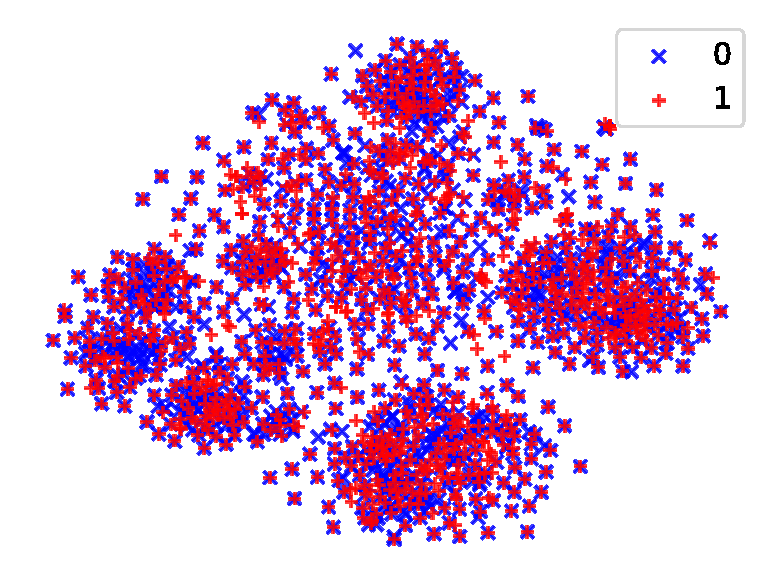
\includegraphics[width=3.5cm]{./images/ca_pre_c.pdf}
	\end{minipage}
	\begin{minipage}{0.45\linewidth}
		\centering
		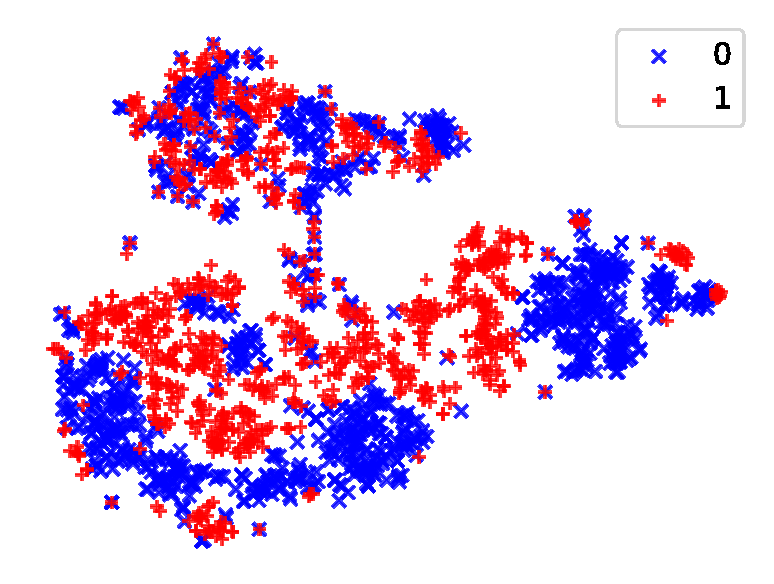
\includegraphics[width=3.5cm]{./images/ca_pre_s.pdf}
	\end{minipage}
	\underline{\small ST$^2$-CrossAlign}\\
	\begin{minipage}{0.45\linewidth}
		\centering
		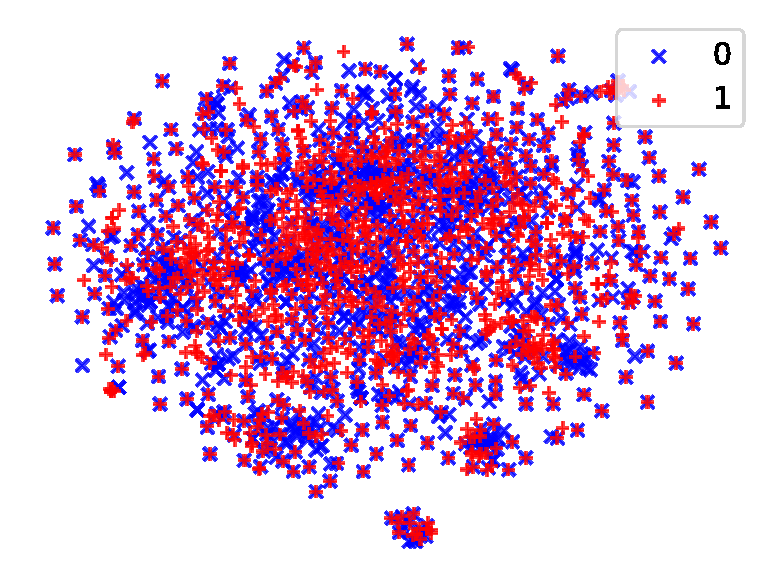
\includegraphics[width=3.5cm]{./images/ca_maml_c.pdf}
	\end{minipage}
	\begin{minipage}{0.45\linewidth}
		\centering
		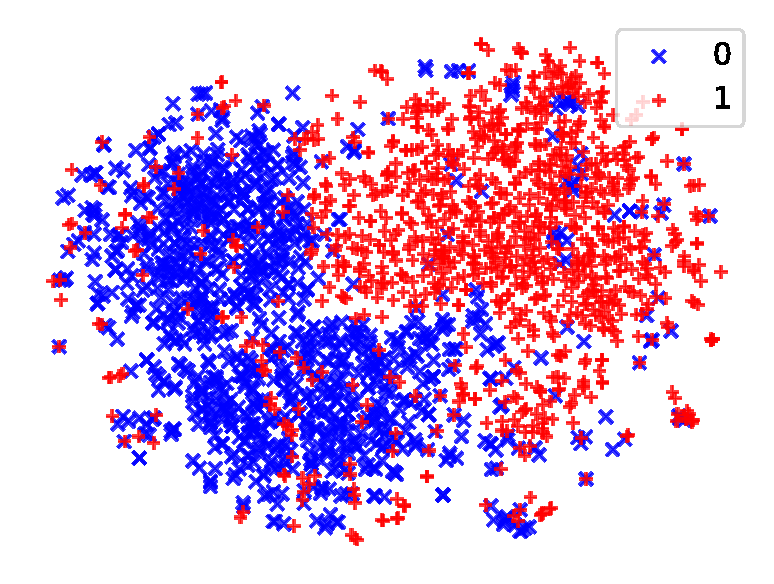
\includegraphics[width=3.5cm]{./images/ca_maml_s.pdf}
	\end{minipage}
	\underline{\small Pretrained VAE}\\
	\begin{minipage}{0.45\linewidth}
		\centering
		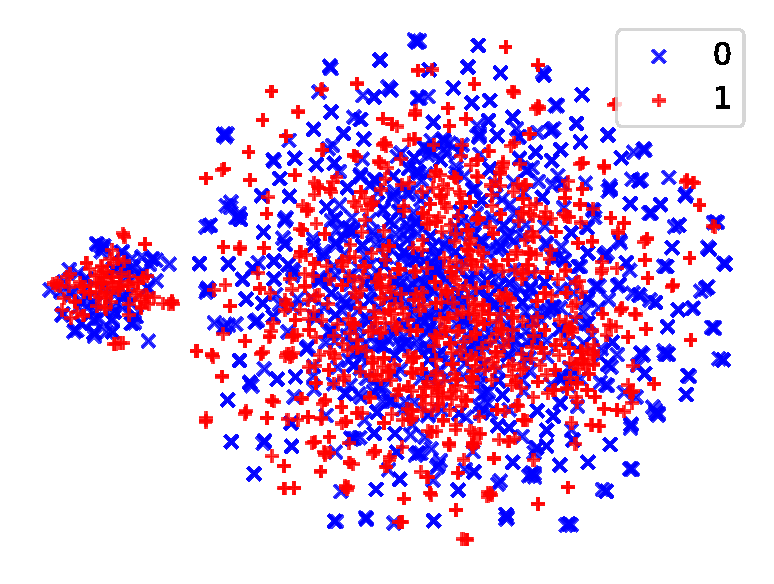
\includegraphics[width=3.5cm]{./images/vae_pre_c.pdf}
	\end{minipage}
	\begin{minipage}{0.45\linewidth}
		\centering
		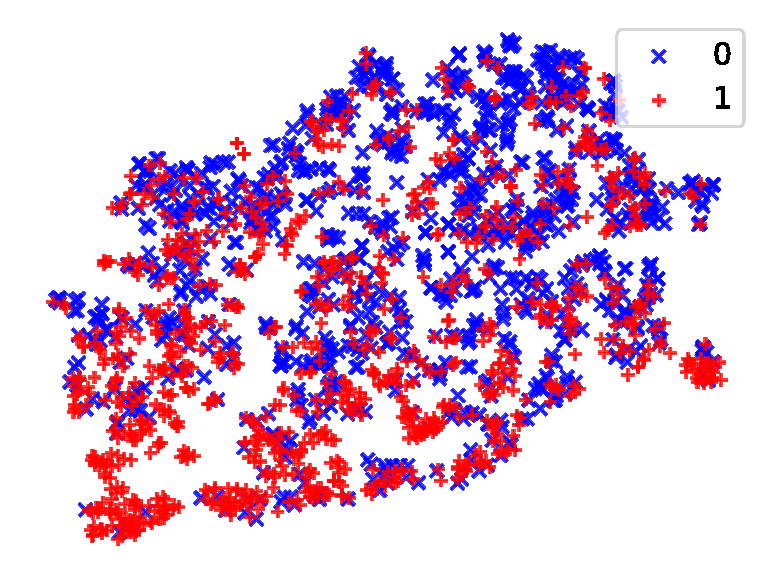
\includegraphics[width=3.5cm]{./images/vae_pre_s.pdf}
	\end{minipage}
	\underline{\small ST$^2$-VAE}\\
	\begin{minipage}{0.45\linewidth}
		\centering
		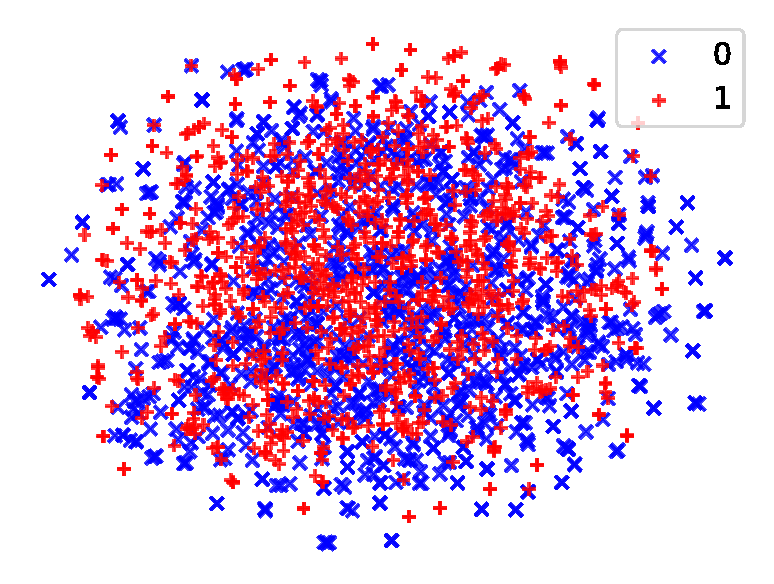
\includegraphics[width=3.5cm]{./images/vae_maml_c.pdf}
	\end{minipage}
	\begin{minipage}{0.45\linewidth}
		\centering
		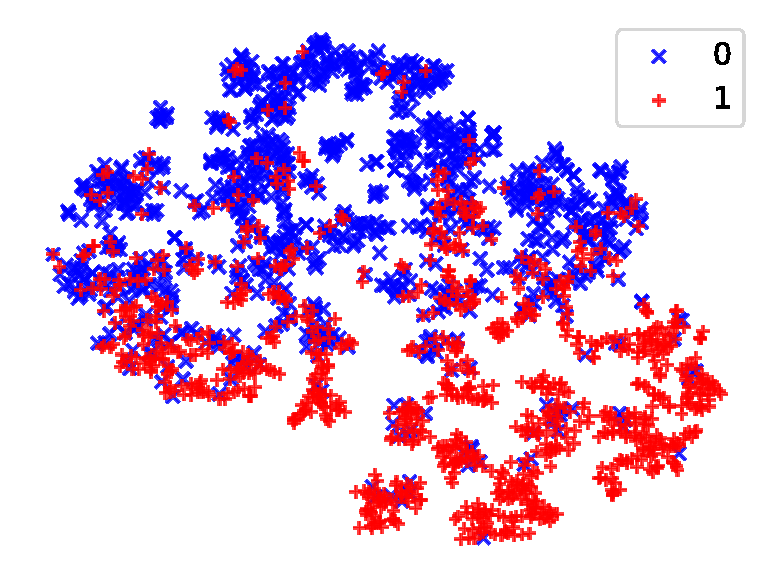
\includegraphics[width=3.5cm]{./images/vae_maml_s.pdf}
	\end{minipage}
	\caption{t-SNE plots for content(left) and style(right) embedding}\label{fig:tsne}
\end{figure}


These two models, together with our ST$^2$ models attempt to disentangle style and content in latent space, and thus is well suited for this experiment, while it is unreasonable to treat hidden state vectors in other baseline models as content/style embedding. Therefore, they are excluded from this experiment.

As we can see from the figures, the content space learned by all models are relatively clustered, while the style spaces are more separated in our ST$^2$ models than the pretrained base models. This verifies that the improvements of meta-learning framework is not limited to a better language model, but also in terms of the disentanglement of styles.


